% Instructions to change to html version:
% Comment out:
%  minipage, multicols,columnbreak, mathbf, hrule
% Replace all: \begin{minipage}% \end{minipage} %\begin{mulicols}  %\end{mulicols}  %\columnbreak % \begin{framed} %\end{framed} %%\hrule
% Search for \mathbf
% Replace $$ with \[ and $ with \(
% Enclose graphics in figure environments and add captions
% Re-tag \df environments as sections, subsections, etc.
% Command Line Code to Create html version:
%First: pdflatex -shell-escape filename.tex                                   
%Second, for each figure: inkscape "filename-figure1.pdf" -o "filename-figure1.png"
% Third: htlatex filename.tex "ht5mjlatex.cfg, charset=utf-8" " -cunihtf -utf8"

\documentclass[10pt]{article}

%\usepackage{tikz, pgf,pgfplots,wasysym,array}
%\usepackage{wasysym,array}

\usepackage{amsmath,amssymb}

\ifdefined\HCode
  \def\pgfsysdriver{pgfsys-tex4ht-updated.def}
\fi 
%\ifdefined\HCode
%  \def\pgfsysdriver{pgfsys-dvisvgm4ht.def}
%\fi 
\usepackage{tikz}
\usetikzlibrary{calc,decorations.markings,arrows}
\usepackage{pgfplots}

\pgfplotsset{compat=1.12}
\usepackage{myexternalize}
\usetikzlibrary{calc,decorations.markings,arrows}
\usepackage{framed}
\usepackage[none]{hyphenat}

\input{../../../common/1336_header_test.tex}
\begin{document}


\everymath{\displaystyle}

\renewcommand{\myTitle}{MATH 1336: Calculus III}

\renewcommand{\mySubTitle}{Section 1.3:  Polar Coordinates}
%~\hfill Name: \underline{~~~~~~~~~~~~~~~~~~~~~~~~~~~~~~~~~~~~~~~~~~~~~~~}



\lectTitle{\vspace*{-.5in}\myTitle}{\vspace*{.1in}\mySubTitle \vspace*{-.25in}}


\setlength{\columnseprule}{0.4pt}
\setlength{\columnsep}{3em}

%\hspace*{-.8in}%\begin{minipage}{1.25\textwidth}
%\begin{framed}

\section*{Intro to Polar Coordinates:}




%\begin{minipage}{.4\textwidth}

\begin{figure}[!h]

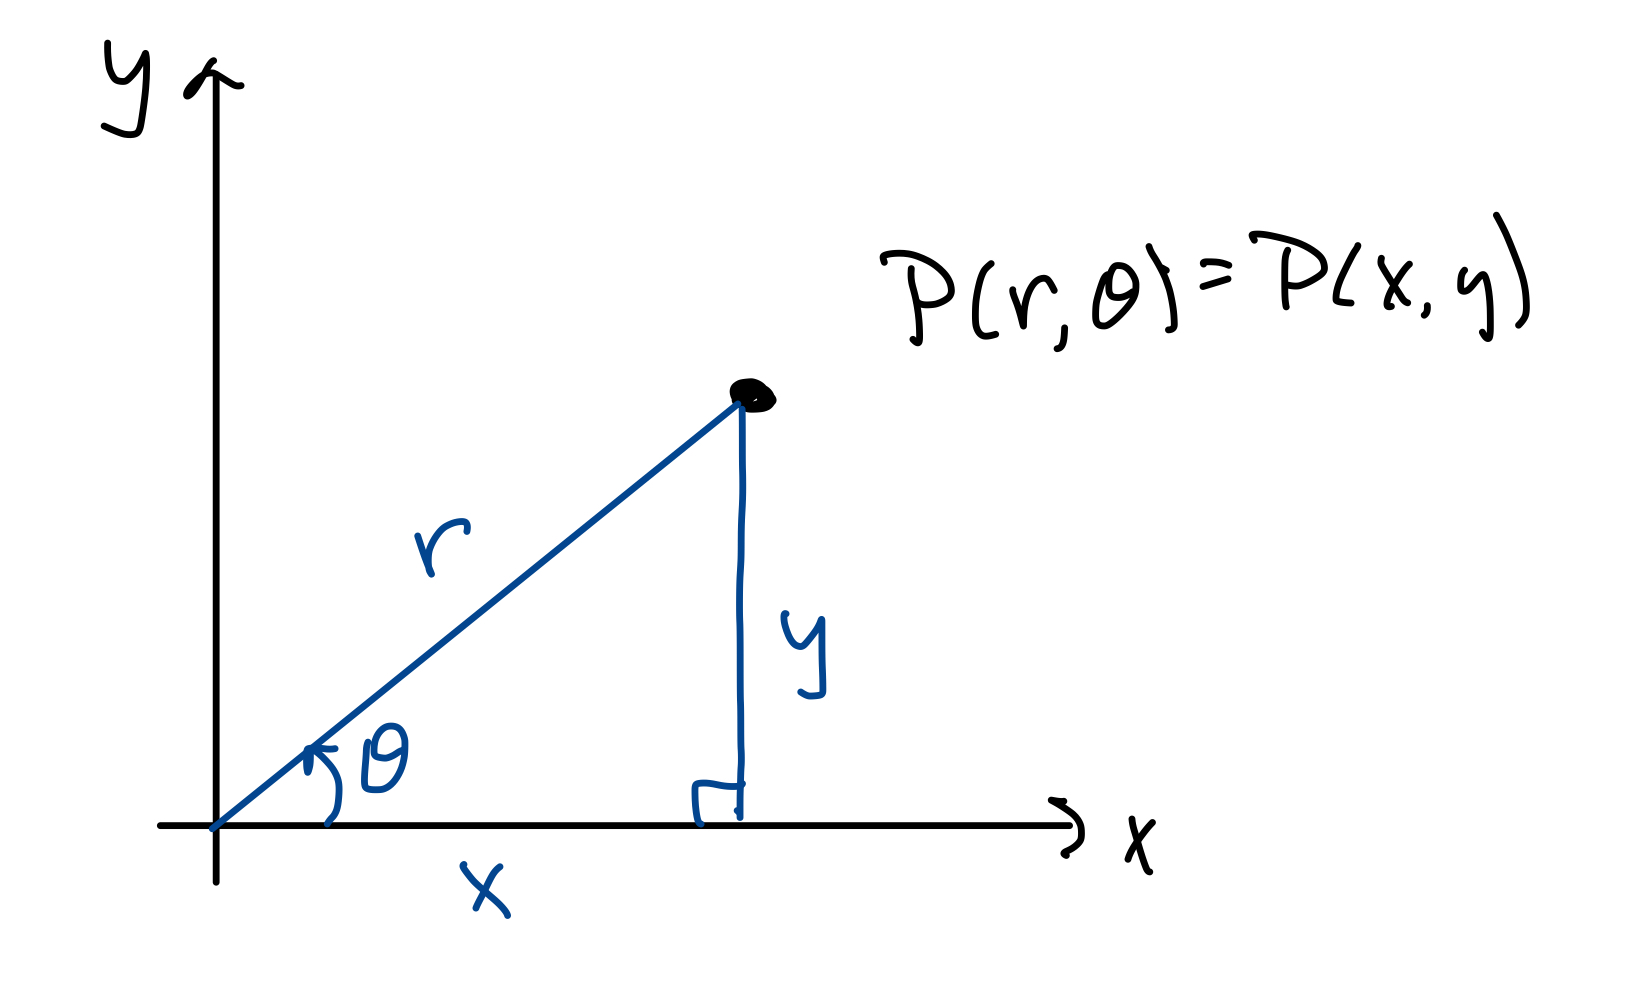
\includegraphics[height=2in]{Ch12s3-Polar-Coordinates.jpeg}\\

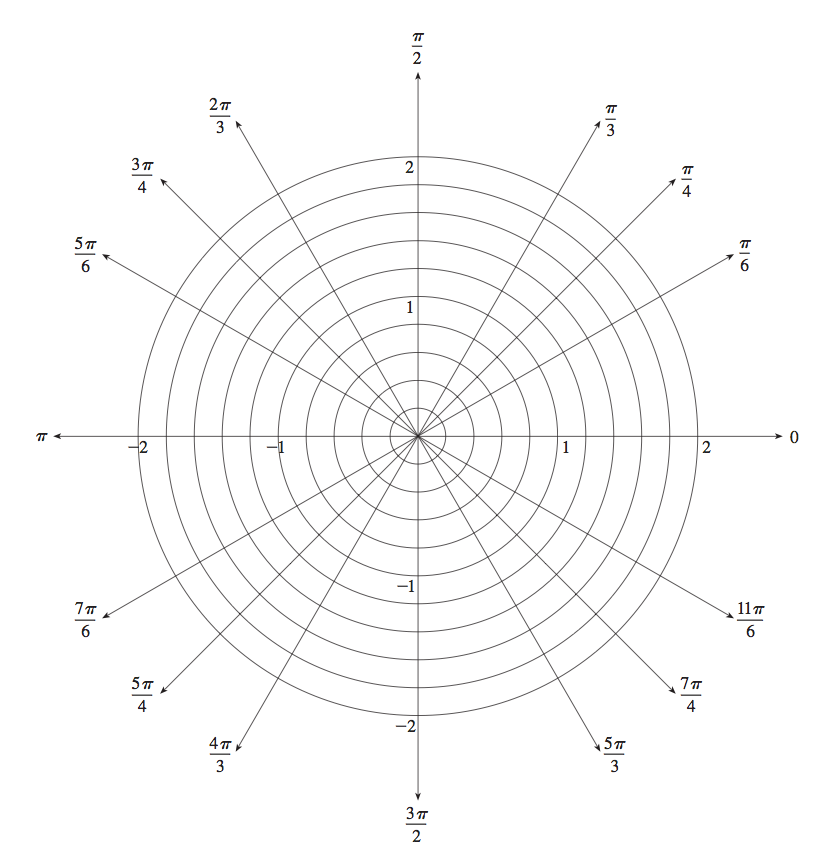
\includegraphics[height=2in]{PolarPaper.png}

\caption{Top: Diagram illustrating the relationship between Polar and Cartesian Coordinates. Bottom: Polar graph paper.}
\end{figure}

%\end{minipage}
\hspace*{.2in}
%\begin{minipage}{.5\textwidth}

Instead of describing points in terms of \(x\) and \(y\) coordinates, use:\\

\(r\): the \textit{signed} distance from the origin\\
\(\theta\): the angle measured counter-clockwise from the \(x\)-axis.\\


\textbf{Note that in this context, we use the convention that \(r\) is a \textit{signed} distance, meaning that it may be positive or negative.}\\

 This allows us to generate more interesting graphs, and also gives us more ways to describe the same point in space.\\


To translate back and forth between polar and Cartesian coordinates, we can use the following equations:

\[x=r \cos\theta, \qquad y=r\sin\theta, \qquad x^2 + y^2 = r^2, \qquad \tan \theta = \frac{y}{x}\]



%\end{minipage}

%\vspace*{.1in}
%%\hrule
%\vspace*{.1in}

%\begin{minipage}{.4\textwidth}
%
%
%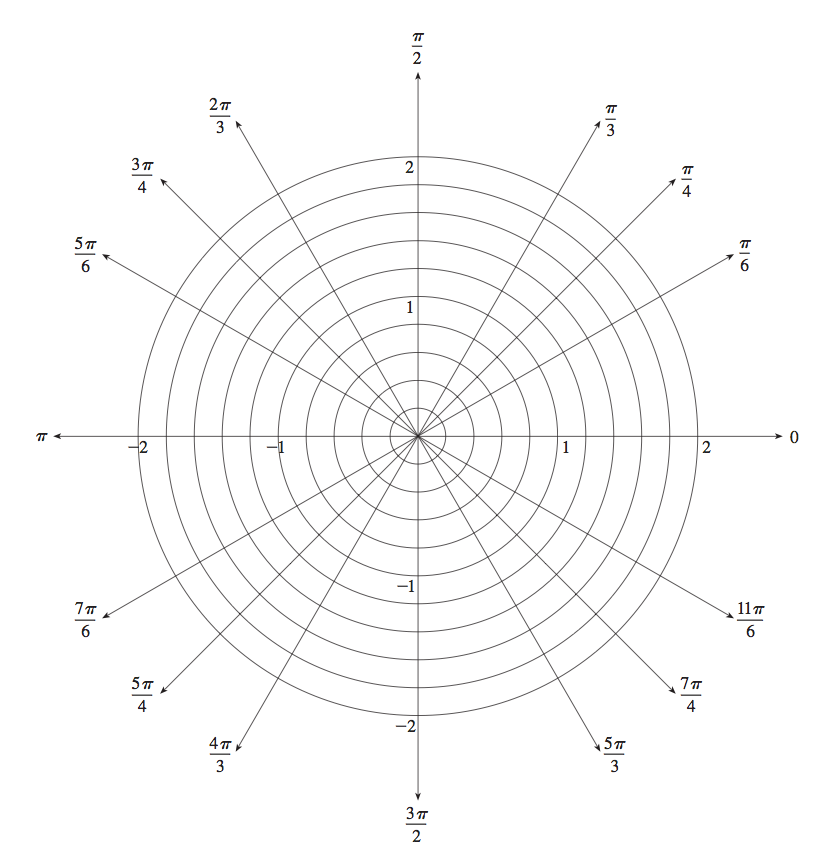
\includegraphics[width=\textwidth]{PolarPaper}
%
%\end{minipage}
%\hspace*{.2in}
%\begin{minipage}{.5\textwidth}

\textbf{Polar Curves:}\\
Given a polar equation \(r = f(\theta)\), the graph is the set of all points that have at least one representation \((r,\theta)\) that satisfies the equation given.\\~\\

\textbf{Tangents to Polar Curves:}

To find an expression for the slope of a polar curve, we start with our expression for the slope of a parametric curve, letting \(\theta\) be the parameter, and then apply the product rule for derivatives:

\[
\frac{dy}{dx} = \frac{\dfrac{dy}{d\theta}}{\dfrac{dx}{d\theta}} = 
 \frac{\dfrac{d}{d\theta}\left(r(\theta)\sin(\theta)\right)}{\dfrac{d}{d\theta}\left(r(\theta)\cos(\theta)\right)} = 
\frac{\dfrac{dr}{d\theta}\sin\theta + r \cos\theta}{\dfrac{dr}{d\theta}\cos\theta - r\sin\theta}
\]

%\vspace*{-.2in}
%\end{minipage}

%\endframed}
%\end{minipage}

\section*{Warm-up Problem:}

\begin{enumerate}

\item On the polar axes above, plot and label the point \(P\) whose polar coordinates are \((r,\theta)=(2, \tfrac{3\pi}{4})\).

\vspace*{.1in}

\item  Find \textbf{two} other pairs of polar coordinates for this point, one with \(r>0\), and one with \(r<0\).

\vspace*{.2in}

\underline{\((r,\theta) = \qquad \qquad \qquad\)} \hfill \underline{\((r,\theta) = \qquad \qquad \qquad\)}

\vspace*{.1in}


\item   Find the Cartesian Coordinates of this point. \textbf{Please leave your answer in \textbf{exact form}}.

\vspace*{.2in}

\underline{\((x,y) = \qquad \qquad \qquad \qquad \qquad \qquad\)}

\end{enumerate}

\pagebreak

%\vspace*{-.6in}
%\begin{framed}
%\vspace*{-.1in}
%\begin{multicols}{2}
%\underline{\textbf{\Large Polar Coordinates:}}
%\begin{eqnarray*}
%x &=& r \cos \theta\\
%y &=& r \sin \theta\\
%&&\\
%r^2 &=& x^2 + y^2\\
%\tan\theta &=&\frac{y}{x}
%\end{eqnarray*}
%\columnbreak
%
%\underline{\textbf{\Large Tangents to Polar Curves:}}
%\begin{eqnarray*}
%\frac{dy}{dx} = \frac{\dfrac{dy}{d\theta}}{\dfrac{dx}{d\theta}} = \frac{\dfrac{dr}{d\theta}\sin\theta + r \cos\theta}{\dfrac{dr}{d\theta}\cos\theta - r\sin\theta}
%\end{eqnarray*}
%\end{multicols}
%\vspace*{-.3in}
%\end{framed}


%\textbf{Example 1:} \hspace*{.4\textwidth} \textbf{Example 2:}\\
%\begin{multicols}{2}
%\noindent\textbf{Example 1:}\\
%Plot the following points on the axes below, then give another pair of polar coordinates that describe the same point.\\
%\(\qquad A: (1,\frac{5\pi}{4}) \qquad \qquad \qquad \qquad \qquad \qquad \qquad \qquad B: (2,-\frac{\pi}{3})\)\\
%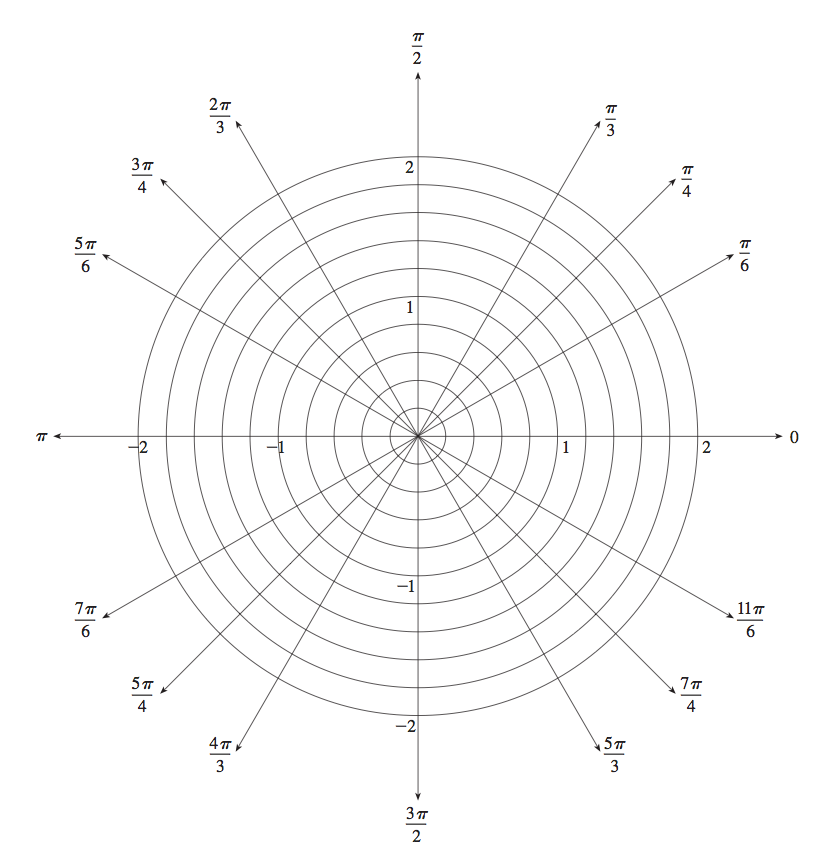
\includegraphics[width=.5\textwidth]{PolarPaper.png} 
%
%%\columnbreak
%
%\noindent \textbf{Example 2:}\\
%Graph the polar curves described by the following equations.\\
%\(r =1 , \qquad r=2, \qquad r=1.5\)\\
%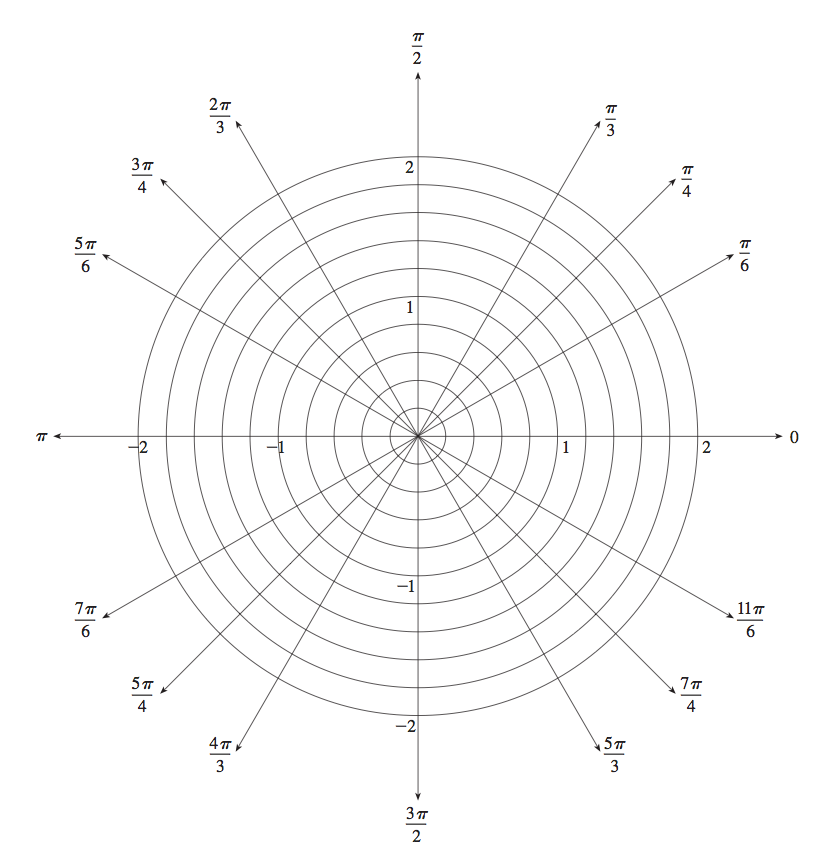
\includegraphics[width=.5\textwidth]{PolarPaper.png}
%\vspace*{-.5in}
%%\end{multicols}
%\pagebreak

\section*{Examples:}

We will work through Example 3 together, then work on the remaining problems in small groups.

\begin{enumerate}[{Example} 1:]

\addtocounter{enumi}{2}

%\noindent\textbf{Example 3:} \\
\item 
Plot the curve \(r=\sin\theta\). \\
\textit{Hint:} Start by creating a table of values for \(\theta\) and \(r\), then plot the points on the axes below.\label{ex3}
\begin{figure}[!h]

\noindent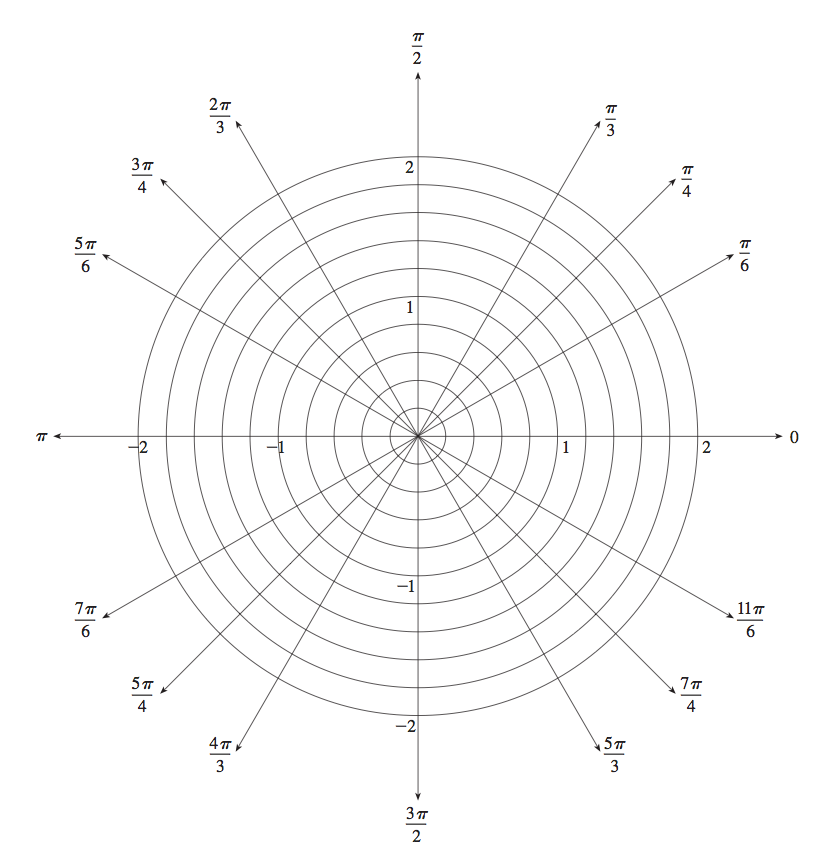
\includegraphics[width=.5\textwidth]{PolarPaper.png} 
\caption{Polar graph paper to be used for Example \ref{ex3}.}
\end{figure}


%\noindent\textbf{Example 4:}\\
\item 
Plot \(r=\theta\) and determine the slope at \(\theta = \frac{\pi}{2}\).\label{ex4}

\begin{figure}[!h]


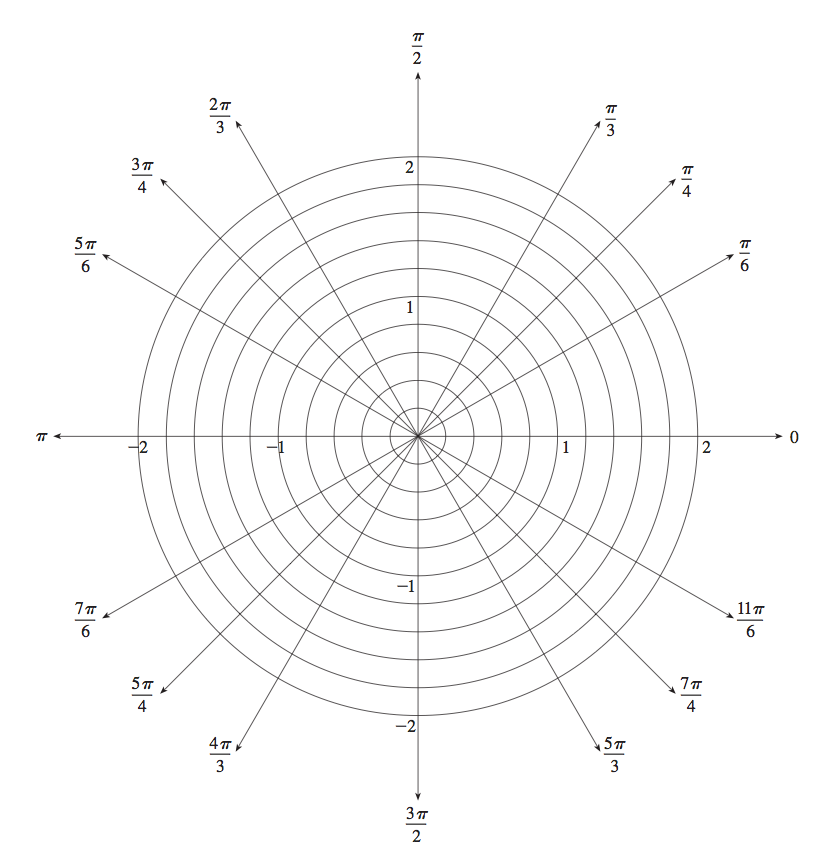
\includegraphics[width=.5\textwidth]{PolarPaper.png}
\caption{Polar graph paper to be used for Example \ref{ex4}.}
\end{figure}

%\vspace*{-.5in}

\vfill

\pagebreak

%\textbf{Example 5:}\\
\item 
Find a polar equation for the curve represented by the given Cartesian equation.
\[
y^2 = 4x
\]

\vfill

%\textbf{Example 6:}\\
\item 
Find a Cartesian equation for the curve represented by the given polar equation.
\[
r = 2 \sec\theta
\]

\vfill

%\textbf{Example 7:}\\
\item 
Find a Cartesian equation for the curve represented by the given polar equation.
\[
r = 2(1+ \cos\theta)
\]

\vfill

\end{enumerate}

\end{document}
